\chapter{What is a Proof?}
\begin{pr}\leavevmode
    \begin{enumerate}[label=\textbf{(\alph*)}]
        \item \label{1.a.sec1} Colors of the triangles are arbitrary since I
        do not remember the exact ones in the text.
        \vspace{1cm}

        
\begin{tikzpicture}
            \draw[fill=red!70] (0,0) -- (5,0) -- ++(-90:1.3) -- cycle;
            \draw[fill=yellow!70] (5,0) -- (5,-5) -- ++(165: 1.3) -- cycle;
            \draw[fill=green!70] (5,-5) -- (0,-5) -- ++(90:1.3) -- cycle;
            \draw[fill=blue!70] (0,-5) -- (0,0) -- ++(-15:1.3) -- cycle;
        \end{tikzpicture}

        \vspace{1.5\baselineskip}
        The middle square is a square of $(b-a) \times (b-a)$

        \item \label{1.b.sec1} $[$\note{Possible Errata:} Arrange the same shapes so they form
        two rectangles, both $a \times b$.$]$

        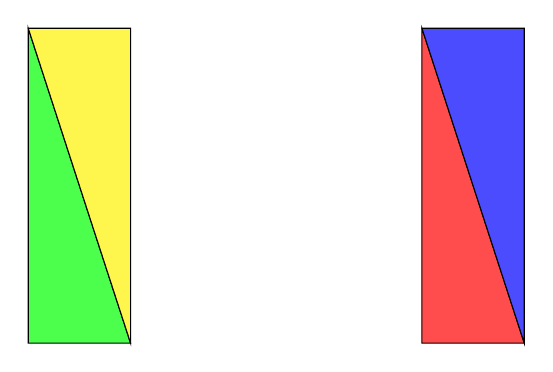
\begin{tikzpicture}
            \begin{scope}
                \draw[fill=green!70] (0,0) -- ++(0,-4) -- ++(1.3,0) -- cycle;
                \draw[fill=yellow!70] (0,0) -- ++(1.3,0) -- ++(0,-4) -- cycle;
            \end{scope}
            \begin{scope}[xshift=5cm]
                \draw[fill=red!70] (0,0) -- ++(0,-4) -- ++(1.3,0) -- cycle;
                \draw[fill=blue!70] (0,0) -- ++(1.3,0) -- ++(0,-4) -- cycle;
            \end{scope}
        \end{tikzpicture}

        We prove by construct a chain of iffs.
        \begin{IEEEeqnarray*}{C'rCl}
            & (b - a)^2 & = & c^2 - 2ab \\
            \Leftrightarrow & a^2 + b^2 - 2ab & = & c^2 - 2ab \\
            \Leftrightarrow & a^2 + b^2 & = & c^2 \\
        \end{IEEEeqnarray*}

        \item The equation would still hold true since $a = b$ is not
        a requirement for the proof. In fact, note that if $a = b$,
        the area of the bigger square in \ref{1.a.sec1} will now be
        exactly equal to the sum of area of all triangles inside it,
        which is equal to the sum of area of two smaller squares in \ref{1.b.sec1}.
        That is, $c^2 = a^2 + b^2$.

        \item Some assumptions about right triangles, squares and lines are,
        \begin{itemize}
            \item 4 identical right triangles.
            \item For every 2 points, there is a line.
        \end{itemize}
    \end{enumerate}
\end{pr}

\begin{pr}\leavevmode
    \begin{enumerate}[label=\textbf{(\alph*)}]
        \item Mistake:
        \begin{equation*}
            \sqrt{(-1)(-1)} = \sqrt{-1}\sqrt{-1}
        \end{equation*}
        The right-hand side of this equation is undefined while the left-hand side
        is defined.
        \item Suppose $1 = -1$, then
        \begin{IEEEeqnarray*}{C'rCl}
                        & 0     & = & 0 \\
            \Rightarrow & 1^2 - 1^2 & = & 1 + 1 \\
            \Rightarrow & (1 - 1)(1 + 1) & = & 1 + 1
        \end{IEEEeqnarray*}
        At this stage, we cancel off $1 + 1$ on each side since they are non-zero, the equation
        then becomes,
        \begin{IEEEeqnarray*}{C'rCl}
            \Rightarrow & 1 - 1 & = & 1 \\
            \Rightarrow & 1 + 1 & = & 1 \\
            \Rightarrow & 2 & = & 1
        \end{IEEEeqnarray*}
        where the second equation is by the antecedent $1 = -1$. Hence, we have
        proved $2 = 1$.
        \item We shall prove the following lemma,
        \begin{lemPr}
            If $r,s > 0$, then $\sqrt{rs} = \sqrt{r}\sqrt{s}$
        \end{lemPr}
        \begin{proof}
            Assume $r,s > 0$. For every positive integer $x$, there is one $\sqrt{x} > 0$
            such that $x = (\sqrt{x})^2$; therefore,
            \begin{equation}
                (\sqrt{r})^2(\sqrt{s})^2 = rs
            \end{equation}
            By commutative and associative property of multiplication, 
            \begin{equation}
                (\sqrt{r})^2(\sqrt{s})^2 = (\sqrt{r}\sqrt{s})^2
            \end{equation}
            which leads to
            \begin{equation}
                (\sqrt{r}\sqrt{s})^2 = rs
            \end{equation}
            Since $rs > 0$, there is also one $\sqrt{rs} > 0$ such that
            $(\sqrt{rs})^2 = rs$. Therefore,
            \begin{equation}
                (\sqrt{r}\sqrt{s})^2 = (\sqrt{rs})^2
            \end{equation}
            Since $\sqrt{r}\sqrt{s} > 0$ and $\sqrt{rs} > 0$,
            we conclude
            \begin{equation}
                \sqrt{r}\sqrt{s} = \sqrt{rs}
            \end{equation}
        \end{proof}
    \end{enumerate}
\end{pr}

\begin{pr}\leavevmode
    \begin{enumerate}[label=\textbf{(\alph*)}]
        \item Mistake,
        \begin{IEEEeqnarray*}{rCl}
            3                & > & 2 \\
            3\log_{10} (1/2) & > & 2\log_{10} (1/2)
        \end{IEEEeqnarray*}
        since $\log_{10} n \;\forall  0 < n < 1$ is always negative.
        \item Wrong because all arithmetic operations must be done
        on numbers with the same currency, so that they will be in the
        same field.
        \item Since $a = b$, $a - b = 0$, and therefore we cannot
        cancel $a - b$ on both sides since we cannot divide each side by $0$.
    \end{enumerate}
\end{pr}

\begin{pr}
    The questionable step is from step 2 to step 3, namely,
    \begin{IEEEeqnarray*}{rCl}
        a + b & \overset{?}{\geq} & 2\sqrt{ab} \\
        a^2 + 2ab + b^2 & \overset{?}{\geq} & 4ab
    \end{IEEEeqnarray*}

    Assume that $a, b < 0$. Then even though the first inequality
    is false, the second inequality is true, which will lead to all
    subsequent inequalities to be true. Therefore, we have just ``proved''
    that arithmetic mean is at least as large as geometric mean for
    all negative numbers $a, b$!

    To fix this,
    \begin{IEEEeqnarray*}{rCl}
        \dfrac{a + b}{2} & \geq & \sqrt{ab} \\
        a + b - 2\sqrt{ab} & \geq & 0 \\
        (\sqrt{a} - \sqrt{b})^2 & \geq & 0 \\
    \end{IEEEeqnarray*}

    This ensures that $a, b \geq 0$ so that the last inequality
    can be defined.
\end{pr}

\begin{pr}\leavevmode
    \\
    The reasoning is wrong because of the implicit assumption
    on Monday.

    \begin{assPr} \label{assPr:1.5:sec1}
        If Albert didn't give the quiz \boldText{before} Monday,
        by Midnight Sunday, we know the quiz has to be on Monday.
    \end{assPr}

    The contrapositive of this statement is,

    \begin{assPr}[equivalent to \ref{assPr:1.5:sec1}]
        If the quiz is not on Monday, then Albert gave the quiz
        \boldText{before} Monday.
    \end{assPr}

    This is a false assumption since we know Albert gives out
    his quiz on next week. This collapses the chain of arguments
    and therefore the reasoning is false.
\end{pr}

\begin{pr}\leavevmode
    \\
    We prove by case analysis. Let $x = \log_{7} n \;\forall n \in \mathbb{Z}^{+}$
    so that $7^x = n$.
    We argue that there are two scenarios,
    \begin{enumerate}
        \item $x$ is an integer
        \item $x$ is a non-integer
    \end{enumerate}
    These cases are clearly exhaustive.
    \begin{casesp}
        \item $x$ is an integer
        
        We use a certain fact called the fundamental theorem of algebra,

        \begin{factPr} \label{fact1:sec1.6:ch1}
            All positive integers are products of unique primes.
        \end{factPr}

        Therefore, for all $n$ that are a product of $7s$ (e.g, $7$, $7^2$, $7^3$, \ldots),
        $x$ is an integer.
        
        \item $x$ is a non-integer
        
        We prove by contradiction. Assume $x$ is rational, then $x = \dfrac{p}{q}$
        for all integers $p,q \in \mathbb{Z}^{+}$ that do not share common factor such that $7^{\frac{p}{q}} = n$.
        Then $n^q = 7^p$. By fact \ref{fact1:sec1.6:ch1}, $n = 7^k$ for some positive integer $k$,
        which means $7^{qk} = 7^p$. Then $\dfrac{p}{q} = k$, which contradicts the fact $p$
        and $q$ do not share a common factor. We conclude that $x$ is irrational.
    \end{casesp}
\end{pr}

\begin{pr}\leavevmode
    \begin{casesp}
        \item $r \geq s$
        
        \begin{equation*}
            max(r,s) + min(r,s) = r + s
        \end{equation*}

        \item $r < s$
        
        \begin{equation*}
            max(r,s) + min(r,s) = s + r = r + s
        \end{equation*}
    \end{casesp}
\end{pr}

\begin{pr}\leavevmode
    \\
    We claim that,

    \begin{claimPr}
        An irrational number powered to an irrational number can be rational.
    \end{claimPr}

    We prove by case analysis. Let's consider $\sqrt{2}^{\sqrt{2}}$ to be one of the two cases,

    \begin{enumerate}
        \item $\sqrt{2}^{\sqrt{2}}$ is rational
        \item $\sqrt{2}^{\sqrt{2}}$ is irrational
    \end{enumerate}

    In case 1, we have the conclusion. In case 2, suppose $x = \sqrt{2}^{\sqrt{2}}$
    and $y = \sqrt{2}$, then

    \begin{equation*}
        x^y = \sqrt{2}^{(\sqrt{2})^2} = (\sqrt{2})^2 = 2
    \end{equation*}

    Therefore, we conclude that an irrational number powered to an irrational number
    can be rational.
\end{pr}

\begin{pr}\leavevmode
    \\
    We prove $|r + s| \leq |r| + |s| \;\forall r,s \in \mathbb{R}$ by case analysis.
    \begin{casesp}
        \item $r > 0$, $s > 0$
        \begin{equation*}
            (r + s) = r + s
        \end{equation*}
        \item $r > 0$, $s < 0$
        \begin{equation*}
            |r + s| \leq r - s
        \end{equation*}
        There are two subcases in this one,
        \begin{casesp}
            \item $r + s \geq 0$
            \begin{equation*}
                r + s < r - s
            \end{equation*}
            \item $r + s < 0$
            \begin{equation*}
                -r - s < r - s
            \end{equation*}
        \end{casesp}
        \item $r < 0$, $s > 0$

        Very similar to the case above, interchange the role of $r, s$.
        
        \item $r < 0$, $s < 0$
        
        Then $-(r + s) = -r - s = (-r) + (-s)$.
    \end{casesp}
\end{pr}

\begin{pr}\leavevmode
    \begin{enumerate}[label=\textbf{(\alph*)}]
        \item We prove by case analysis. Without loss of generality, assume $z = a + b$
        and $d = z + c$ where $a,b,c,d \in \mathbb{Z}^{+}$, then
        one of the following four cases happens,

        \begin{casesp}
            \item $z$ is odd and $c$ is odd
            
            $z$ is odd IFF one and only one of the summands is even and the other is odd.
            In this case, $d$ is even if one of $a,b,c$ is even.

            \item $z$ is even and $c$ is even
            
            For $z$ to be even, there are two sub-cases,

            \begin{casesp}
                \item Both $a$ and $b$ are evens
                
                $d$ is even if all of $a,b,c$ are even.
                \item Both $a$ and $b$ are odds
                
                $d$ is even if one and only one of $a,b,c$ is even.
            \end{casesp}

            \item $z$ is even and $c$ is odd
            
            $d$ is odd in this case.

            \item $z$ is odd and $c$ is even
            
            $d$ is also odd in this case.
        \end{casesp}

        We conclude that $d$ is even IFF either one and only one of $a,b,c$
        is even or all $a,b,c$ are evens.

        \item We shall first prove a lemma,
        
        \begin{lemPr}
            If $x$ is even, $x^2$ is a multiple of $4$.
            If $x$ is odd, $x^2$ is one more than a multiple of $4$.
        \end{lemPr}
        \begin{proof}
            If $x$ is even, $x = 2k$ for some integer $k$, then $x^2 = 4k^2$.
            If $x$ is odd, $x = 2m + 1$ for some integer $m$, then $x^2 = 4(m^2 + m) + 1$.
        \end{proof}

        Suppose,
        \begin{equation*}
            w^2 + x^2 + y^2 = z^2
        \end{equation*}
        for all $w,x,y,z \in \mathbb{Z}^{+}$.
        We shall prove the statement,
        \begin{theoPr}
            $z$ is even IFF all $w,x,y$ are even.
        \end{theoPr}
        \begin{proof}
            We shall prove by case analysis. Assume if $w,x,y$ are even, then
            $w = 2i, x = 2j, y = 2k$ for some integer $i, j, k$; if $w,x,y$
            are odd, then $w = 2m + 1, x = 2n + 1, y = 2l + 1$ for some integer
            $m, n, l$. Then one of the following four cases happen,

            \begin{casesp}
                \item All $w,x,y$ are odd
                \begin{IEEEeqnarray*}{rCl}
                    z^2 & = & (2m + 1)^2 + (2n + 1)^2 + (2l + 1)^2 \\
                    & = & 4(m^2 + n^2 + l^2 + m + n + l) + 3
                \end{IEEEeqnarray*}

                \item One of $w,x,y$ is even
                \begin{IEEEeqnarray*}{rCl}
                    z^2 & = & (2i)^2 + (2n + 1)^2 + (2l + 1)^2 \\
                        & = & 4(i^2 + n^2 + l^2 + n + l) + 2
                \end{IEEEeqnarray*}

                \item Two of $w,x,y$ are even
                \begin{IEEEeqnarray*}{rCl}
                    z^2 & = & (2i)^2 + (2j)^2 + (2l + 1)^2 \\
                        & = & 4(i^2 + j^2 + l^2 + l) + 1
                \end{IEEEeqnarray*}

                \item All of $w,x,y$ are even
                \begin{IEEEeqnarray*}{rCl}
                    z^2 & = & (2i)^2 + (2j)^2 + (2k)^2 \\
                        & = & 4(i^2 + j^2 + k^2)
                \end{IEEEeqnarray*}
            \end{casesp}

            Therefore, if either one and only one of $w,x,y$ is even or all of $w,x,y$
            are even, then $z^2$ is even, which implies $z$ is even. Conversely,
            if $z$ is even, by the above lemma, $z^2$ does not exist in Case 2.
            We conclude that $z$ is even IFF all of $w,x,y$ are even.
        \end{proof}
    \end{enumerate}
\end{pr}

\begin{pr}\leavevmode
    \\
    We want to prove the theorem,
    \begin{theoPr}
        There exists an irrational number $a$ such that $a^{\sqrt{3}}$ is rational.
    \end{theoPr}
    \begin{proof}
        We prove by case analysis. The number $x = \sqrt[3]{2}^{\sqrt{3}}$ must be one of
        the two cases,
        \begin{casesp}
            \item $x$ is rational.
            
            In this case, $a = \sqrt[3]{2}$ and $a$ is irrational.

            \item $x$ is irrational.
            
            Let $a = \sqrt[3]{2}^{\sqrt{3}}$. Then $a$ is irrational such that,

            \begin{IEEEeqnarray*}{rCl}
                a^{\sqrt{3}} & = & (\sqrt[3]{2})^{(\sqrt{3})^2} \\
                             & = & (\sqrt[3]{2})^3 \\
                             & = & 2 
            \end{IEEEeqnarray*}
        \end{casesp}

        We conclude that there exists an irrational $a$ such that $a^{\sqrt{3}}$
        is rational.
    \end{proof}
\end{pr}